\documentclass[letterpaper, 11pt]{extarticle}
% \usepackage{fontspec}

% ==================================================

% document parameters
% \usepackage[spanish, mexico, es-lcroman]{babel}
\usepackage[english]{babel}
\usepackage[margin = 1in]{geometry}

% ==================================================

% Packages for math
\usepackage{mathrsfs}
\usepackage{amsfonts}
\usepackage{amsmath}
\usepackage{amsthm}
\usepackage{amssymb}
\usepackage{physics}
\usepackage{dsfont}
\usepackage{esint}

% ==================================================

% Packages for writing
\usepackage{enumerate}
\usepackage[shortlabels]{enumitem}
\usepackage{framed}
\usepackage{csquotes}

% ==================================================

% Miscellaneous packages
\usepackage{float}
\usepackage{tabularx}
\usepackage{xcolor}
\usepackage{multicol}
\usepackage{subcaption}
\usepackage{caption}
\usepackage{appendix}
\captionsetup{format = hang, margin = 10pt, font = small, labelfont = bf}

% Citation
\usepackage[round, authoryear]{natbib}

% Hyperlinks setup
\usepackage{hyperref}
\definecolor{links}{rgb}{0.36,0.54,0.66}
\hypersetup{
   colorlinks = true,
    linkcolor = black,
     urlcolor = blue,
    citecolor = blue,
    filecolor = blue,
    pdfauthor = {Author},
     pdftitle = {Title},
   pdfsubject = {subject},
  pdfkeywords = {one, two},
  pdfproducer = {LaTeX},
   pdfcreator = {pdfLaTeX},
   }
\usepackage{titlesec}
\usepackage[many]{tcolorbox}

% Adjust spacing after the chapter title
\titlespacing*{\chapter}{0cm}{-2.0cm}{0.50cm}
\titlespacing*{\section}{0cm}{0.50cm}{0.25cm}

% Indent 
\setlength{\parindent}{0pt}
\setlength{\parskip}{1ex}

% --- Theorems, lemma, corollary, postulate, definition ---
% \numberwithin{equation}{section}

\newtcbtheorem[]{problem}{Problem}%
    {enhanced,
    colback = black!5, %white,
    colbacktitle = black!5,
    coltitle = black,
    boxrule = 0pt,
    frame hidden,
    borderline west = {0.5mm}{0.0mm}{black},
    fonttitle = \bfseries\sffamily,
    breakable,
    before skip = 3ex,
    after skip = 3ex
}{problem}

\tcbuselibrary{skins, breakable}

% --- You can define your own color box. Just copy the previous \newtcbtheorm definition and use the colors of yout liking and the title you want to use.
% --- Basic commands ---
%   Euler's constant
\newcommand{\eu}{\mathrm{e}}

%   Imaginary unit
\newcommand{\im}{\mathrm{i}}

%   Sexagesimal degree symbol
\newcommand{\grado}{\,^{\circ}}

% --- Comandos para álgebra lineal ---
% Matrix transpose
\newcommand{\transpose}[1]{{#1}^{\mathsf{T}}}

%%% Comandos para cálculo
%   Definite integral from -\infty to +\infty
\newcommand{\Int}{\int\limits_{-\infty}^{\infty}}

%   Indefinite integral
\newcommand{\rint}[2]{\int{#1}\dd{#2}}

%  Definite integral
\newcommand{\Rint}[4]{\int\limits_{#1}^{#2}{#3}\dd{#4}}

%   Dot product symbol (use the command \bigcdot)
\makeatletter
\newcommand*\bigcdot{\mathpalette\bigcdot@{.5}}
\newcommand*\bigcdot@[2]{\mathbin{\vcenter{\hbox{\scalebox{#2}{$\m@th#1\bullet$}}}}}
\makeatother

%   Hamiltonian
\newcommand{\Ham}{\hat{\mathcal{H}}}

%   Trace
\renewcommand{\Tr}{\mathrm{Tr}}

% Christoffel symbol of the second kind
\newcommand{\christoffelsecond}[4]{\dfrac{1}{2}g^{#3 #4}(\partial_{#1} g_{#2 #4} + \partial_{#2} g_{#1 #4} - \partial_{#4} g_{#1 #2})}

% Riemann curvature tensor
\newcommand{\riemanncurvature}[5]{\partial_{#3} \Gamma_{#4 #2}^{#1} - \partial_{#4} \Gamma_{#3 #2}^{#1} + \Gamma_{#3 #5}^{#1} \Gamma_{#4 #2}^{#5} - \Gamma_{#4 #5}^{#1} \Gamma_{#3 #2}^{#5}}

% Covariant Riemann curvature tensor
\newcommand{\covariantriemanncurvature}[5]{g_{#1 #5} R^{#5}{}_{#2 #3 #4}}

% Ricci tensor
\newcommand{\riccitensor}[5]{g_{#1 #5} R^{#5}{}_{#2 #3 #4}}

\begin{document}

\begin{Large}
    \textsf{\textbf{Stochastic Linear Bandits}}
    An Empirical Study
\end{Large}

\vspace{1ex}

\textsf{\textbf{Students:}} \text{Your names}, \\
\textsf{\textbf{Lecturer:}} \text{Claire Vernade}, Contact me on Slack if anything looks weird, or find my email on my \href{www.cvernade.com}{website} 


\vspace{2ex}

Stochastic Linear Bandits are a great way to model contextual sequential decision making problems. We saw them in class and you can read further in the Bandit book \citep{lattimore2020bandit}. In this assignment, your task will be to implement them in order to discuss concretely their performance on simulated environments. The `companion' notebook is attached in this Overleaf. it contains a boiler plate for the experiments and the main questions you will need to answer below. On my website you can find a sample notebook for K-armed bandits (not linear) that may help you get started. 

\textbf{Hard constraint:} Your report can be at most 3 pages + a possible appendix if you decide to also address the Bonus part at the end of the notebook. Thus, if you need to include code snippets or figures, you will have to carefully choose which ones. You are welcome to (and you should!) delete anything I wrote here and below, as long as you re-introduce enough context for your answers, plots and discussions. The clarity of your presentation will be taken into account in the evaluation. Each additional page ($>3$ for the main part, appendix and references do not count) will count -1 on your grade. 

\begin{problem}{Linear Epsilon Greedy (/5)}{}
\begin{itemize}
    \item Complete the implementation of the Linear Bandit environment and the action generation function;
    \item Implement Linear Epsilon Greedy and test it on a simple problem of your choice. Describe your chosen benchmark, report your results and comment. Is it a strong baseline? 
    \item Discuss the complexity of the matrix inversion step and propose a better, incremental update. Report the gain in runtimes that you observed as a function of $d$.
\end{itemize}
\end{problem}

\begin{problem}{LinUCB and LinTS (/5)}{}
\begin{itemize}
    \item Implement LinUCB and LinTS. 
    \item For Thompson Sampling, what is the posterior at time $t$?
    \item We want to know if there is a better algorithm out of all the ones you implemented. Propose an experiment (describe it) and report your results and conclusions.
\end{itemize}
\end{problem}

\section{Linear Epsilon Greedy}
\subsection{Implementation of Linear Bandit environment and action generation function}
To implement the action generation function we will use fact that if $ X = (X_1, X_2, \ldots, X_n) \sim \mathcal{N}(0, I_n) $, 
then $ Y = X / \sqrt{X_1^2 + \ldots + X_n^2} $ is uniformly distributed on the surface of the unit sphere. It is an immediate
consequence that for $Y$ as defined above and $\mu \in \mathbb{R}^n$, $ Y + \mu$ is uniformly distributed on a sphere with unit radius,
centered at the point $\mu$. With that in mind, we propose the following implementation for the aciton generation function:
\begin{verbatim}
def ActionsGenerator(K,d,mean=None):
  res = np.random.normal(0,1,size=(K, d))
  norms = np.linalg.norm(res,axis=1)
  res /= norms[:,np.newaxis]
  if mean is not None:
    res += mean
  return res
\end{verbatim}
Implementation of the \textbf{LinearBandit} environment is straightforward and can be seen in the appendix.
\subsection{Benchmark of Linear Epsilon Greedy}
\subsection{Performance analysis of different matrix inversion methods for updating the confidence ellipsoid}
We compare three different methods for updating the confidence ellipsoid matrix between timesteps:
\begin{itemize}
  \item classic matrix inversion via \textbf{numpy.linalg.inv} - $\mathcal{O}(d^3)$ time complexity
  \item approximate matrix inversion via \textbf{numpy.linalg.lstsq} - $\mathcal{O}(d^3)$ time complexity
  \item Sherman-Morrison formula for computing the inverse of a matrix after rank-1 update - $\mathcal{O}(d^2)$ time complexity
\end{itemize}
We use two benchmarks to compare the methods. In the first one we observe the runtimes of agents in a number of environments
with a fixed \textit{arm-dimension} $d$ and a varying number of arms $K$. In the second benchmark we switch things up and instead fix $d$
and let $K$ vary. The experiments confirm our intuition that the method based on the Sherman-Morrison formula has the best performance as the
arm-dimension $d$ increases.

\begin{figure}[h!]
  \centering
  % First plot
  \begin{subfigure}[b]{0.45\textwidth}
      \centering
      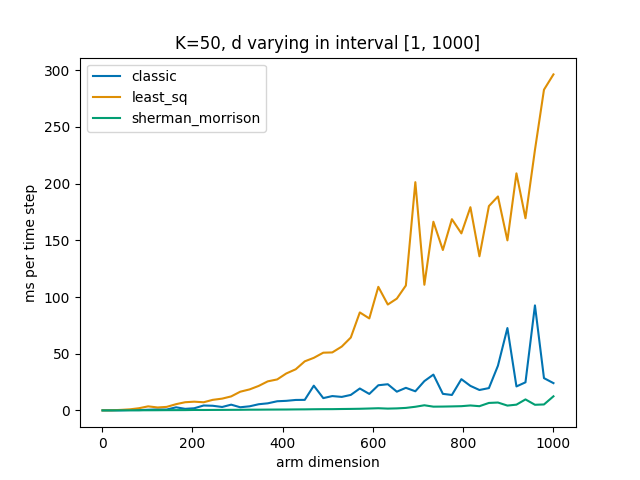
\includegraphics[width=\textwidth]{plots/d_varying_time.png}
      \label{fig:plot1}
  \end{subfigure}
  \hfill
  % Second plot
  \begin{subfigure}[b]{0.45\textwidth}
      \centering
      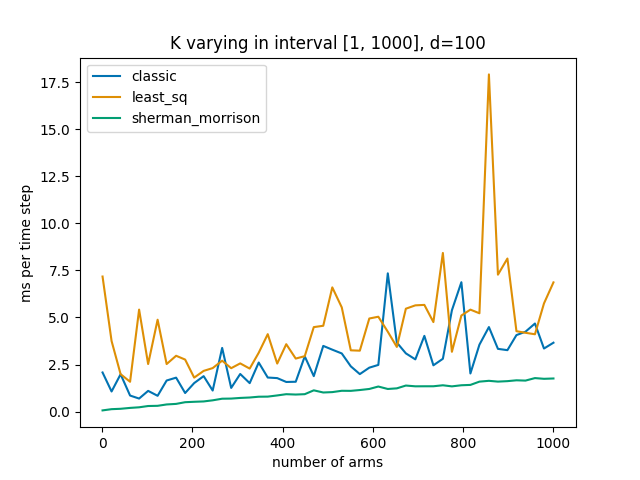
\includegraphics[width=\textwidth]{plots/K_varying_time.png}
      \label{fig:plot2}
  \end{subfigure}
  \label{fig:combined_plots}
\end{figure}


% =================================================

% \newpage

% \vfill
%%% Reminder: Maximum 3 pages
\newpage

\bibliographystyle{apalike}
\bibliography{references}


\appendix

\section{Bonus section: The role of the action set}

This last part allows you to study how certain actions sets can be hard for LinUCB. I propose some code to highlight this phenomenon, that was unveiled by \citet{lattimore2017end}. 
Follow the instructions in the notebook and report your results and comments here. 
\emph{This part can count up to (+2) points, meaning that the maximal grade is (12/10) and could compensate missed points on the Quiz or on the project. }

\section{Implementation of \textbf{Linear Bandit} environment}
\begin{verbatim}
  class LinearBandit:
  def __init__(self, theta, K, var=1., fixed_actions=None):
    """
    theta: d-dimensional vector (bounded) representing the hidden parameter
    K: number of actions per round (random action vectors generated each time)
    pb_type: string in 'fixed', 'iid', 'nsr' (please ignore NotSoRandom)
    """
    self.d = np.size(theta)
    self.theta = theta
    self.K = K
    self.var = var
    self.fixed_actions = fixed_actions
    self.current_action_set = self.get_action_set()

  def get_action_set(self):
    """
    Generates a set of vectors in dimension self.d. Use your ActionsGenerator
    Alternatively, the set of actions is fixed a priori (given as input).
    Implement a condition to return the fixed set when one is given
    """
    if self.fixed_actions is not None:
      return self.fixed_actions
    else:
      self.current_action_set = ActionsGenerator(self.K, self.d)
      return self.current_action_set

  def get_reward(self, action):
    """ sample reward given action and the model of this bandit environment
    action: d-dimensional vector (action chosen by the learner)
    """
    mean = np.dot(action, self.theta)
    return np.random.normal(mean, scale=self.var)

  def get_means(self):
    return np.dot(self.current_action_set, self.theta)
\end{verbatim}


\end{document}